% Options for packages loaded elsewhere
\PassOptionsToPackage{unicode}{hyperref}
\PassOptionsToPackage{hyphens}{url}
\PassOptionsToPackage{dvipsnames,svgnames,x11names}{xcolor}
%
\documentclass[
  letterpaper,
  DIV=11,
  numbers=noendperiod]{scrartcl}

\usepackage{amsmath,amssymb}
\usepackage{iftex}
\ifPDFTeX
  \usepackage[T1]{fontenc}
  \usepackage[utf8]{inputenc}
  \usepackage{textcomp} % provide euro and other symbols
\else % if luatex or xetex
  \usepackage{unicode-math}
  \defaultfontfeatures{Scale=MatchLowercase}
  \defaultfontfeatures[\rmfamily]{Ligatures=TeX,Scale=1}
\fi
\usepackage{lmodern}
\ifPDFTeX\else  
    % xetex/luatex font selection
\fi
% Use upquote if available, for straight quotes in verbatim environments
\IfFileExists{upquote.sty}{\usepackage{upquote}}{}
\IfFileExists{microtype.sty}{% use microtype if available
  \usepackage[]{microtype}
  \UseMicrotypeSet[protrusion]{basicmath} % disable protrusion for tt fonts
}{}
\makeatletter
\@ifundefined{KOMAClassName}{% if non-KOMA class
  \IfFileExists{parskip.sty}{%
    \usepackage{parskip}
  }{% else
    \setlength{\parindent}{0pt}
    \setlength{\parskip}{6pt plus 2pt minus 1pt}}
}{% if KOMA class
  \KOMAoptions{parskip=half}}
\makeatother
\usepackage{xcolor}
\setlength{\emergencystretch}{3em} % prevent overfull lines
\setcounter{secnumdepth}{5}
% Make \paragraph and \subparagraph free-standing
\makeatletter
\ifx\paragraph\undefined\else
  \let\oldparagraph\paragraph
  \renewcommand{\paragraph}{
    \@ifstar
      \xxxParagraphStar
      \xxxParagraphNoStar
  }
  \newcommand{\xxxParagraphStar}[1]{\oldparagraph*{#1}\mbox{}}
  \newcommand{\xxxParagraphNoStar}[1]{\oldparagraph{#1}\mbox{}}
\fi
\ifx\subparagraph\undefined\else
  \let\oldsubparagraph\subparagraph
  \renewcommand{\subparagraph}{
    \@ifstar
      \xxxSubParagraphStar
      \xxxSubParagraphNoStar
  }
  \newcommand{\xxxSubParagraphStar}[1]{\oldsubparagraph*{#1}\mbox{}}
  \newcommand{\xxxSubParagraphNoStar}[1]{\oldsubparagraph{#1}\mbox{}}
\fi
\makeatother

\usepackage{color}
\usepackage{fancyvrb}
\newcommand{\VerbBar}{|}
\newcommand{\VERB}{\Verb[commandchars=\\\{\}]}
\DefineVerbatimEnvironment{Highlighting}{Verbatim}{commandchars=\\\{\}}
% Add ',fontsize=\small' for more characters per line
\usepackage{framed}
\definecolor{shadecolor}{RGB}{241,243,245}
\newenvironment{Shaded}{\begin{snugshade}}{\end{snugshade}}
\newcommand{\AlertTok}[1]{\textcolor[rgb]{0.68,0.00,0.00}{#1}}
\newcommand{\AnnotationTok}[1]{\textcolor[rgb]{0.37,0.37,0.37}{#1}}
\newcommand{\AttributeTok}[1]{\textcolor[rgb]{0.40,0.45,0.13}{#1}}
\newcommand{\BaseNTok}[1]{\textcolor[rgb]{0.68,0.00,0.00}{#1}}
\newcommand{\BuiltInTok}[1]{\textcolor[rgb]{0.00,0.23,0.31}{#1}}
\newcommand{\CharTok}[1]{\textcolor[rgb]{0.13,0.47,0.30}{#1}}
\newcommand{\CommentTok}[1]{\textcolor[rgb]{0.37,0.37,0.37}{#1}}
\newcommand{\CommentVarTok}[1]{\textcolor[rgb]{0.37,0.37,0.37}{\textit{#1}}}
\newcommand{\ConstantTok}[1]{\textcolor[rgb]{0.56,0.35,0.01}{#1}}
\newcommand{\ControlFlowTok}[1]{\textcolor[rgb]{0.00,0.23,0.31}{\textbf{#1}}}
\newcommand{\DataTypeTok}[1]{\textcolor[rgb]{0.68,0.00,0.00}{#1}}
\newcommand{\DecValTok}[1]{\textcolor[rgb]{0.68,0.00,0.00}{#1}}
\newcommand{\DocumentationTok}[1]{\textcolor[rgb]{0.37,0.37,0.37}{\textit{#1}}}
\newcommand{\ErrorTok}[1]{\textcolor[rgb]{0.68,0.00,0.00}{#1}}
\newcommand{\ExtensionTok}[1]{\textcolor[rgb]{0.00,0.23,0.31}{#1}}
\newcommand{\FloatTok}[1]{\textcolor[rgb]{0.68,0.00,0.00}{#1}}
\newcommand{\FunctionTok}[1]{\textcolor[rgb]{0.28,0.35,0.67}{#1}}
\newcommand{\ImportTok}[1]{\textcolor[rgb]{0.00,0.46,0.62}{#1}}
\newcommand{\InformationTok}[1]{\textcolor[rgb]{0.37,0.37,0.37}{#1}}
\newcommand{\KeywordTok}[1]{\textcolor[rgb]{0.00,0.23,0.31}{\textbf{#1}}}
\newcommand{\NormalTok}[1]{\textcolor[rgb]{0.00,0.23,0.31}{#1}}
\newcommand{\OperatorTok}[1]{\textcolor[rgb]{0.37,0.37,0.37}{#1}}
\newcommand{\OtherTok}[1]{\textcolor[rgb]{0.00,0.23,0.31}{#1}}
\newcommand{\PreprocessorTok}[1]{\textcolor[rgb]{0.68,0.00,0.00}{#1}}
\newcommand{\RegionMarkerTok}[1]{\textcolor[rgb]{0.00,0.23,0.31}{#1}}
\newcommand{\SpecialCharTok}[1]{\textcolor[rgb]{0.37,0.37,0.37}{#1}}
\newcommand{\SpecialStringTok}[1]{\textcolor[rgb]{0.13,0.47,0.30}{#1}}
\newcommand{\StringTok}[1]{\textcolor[rgb]{0.13,0.47,0.30}{#1}}
\newcommand{\VariableTok}[1]{\textcolor[rgb]{0.07,0.07,0.07}{#1}}
\newcommand{\VerbatimStringTok}[1]{\textcolor[rgb]{0.13,0.47,0.30}{#1}}
\newcommand{\WarningTok}[1]{\textcolor[rgb]{0.37,0.37,0.37}{\textit{#1}}}

\providecommand{\tightlist}{%
  \setlength{\itemsep}{0pt}\setlength{\parskip}{0pt}}\usepackage{longtable,booktabs,array}
\usepackage{calc} % for calculating minipage widths
% Correct order of tables after \paragraph or \subparagraph
\usepackage{etoolbox}
\makeatletter
\patchcmd\longtable{\par}{\if@noskipsec\mbox{}\fi\par}{}{}
\makeatother
% Allow footnotes in longtable head/foot
\IfFileExists{footnotehyper.sty}{\usepackage{footnotehyper}}{\usepackage{footnote}}
\makesavenoteenv{longtable}
\usepackage{graphicx}
\makeatletter
\newsavebox\pandoc@box
\newcommand*\pandocbounded[1]{% scales image to fit in text height/width
  \sbox\pandoc@box{#1}%
  \Gscale@div\@tempa{\textheight}{\dimexpr\ht\pandoc@box+\dp\pandoc@box\relax}%
  \Gscale@div\@tempb{\linewidth}{\wd\pandoc@box}%
  \ifdim\@tempb\p@<\@tempa\p@\let\@tempa\@tempb\fi% select the smaller of both
  \ifdim\@tempa\p@<\p@\scalebox{\@tempa}{\usebox\pandoc@box}%
  \else\usebox{\pandoc@box}%
  \fi%
}
% Set default figure placement to htbp
\def\fps@figure{htbp}
\makeatother

% load packages
\usepackage{geometry}
\usepackage{xcolor}
\usepackage{eso-pic}
\usepackage{fancyhdr}
\usepackage{sectsty}
\usepackage{fontspec}
\usepackage{titlesec}

%% Set page size with a wider right margin
\geometry{a4paper, total={170mm,257mm}, left=20mm, top=20mm, bottom=20mm, right=50mm}

%% Let's define some colours
\definecolor{light}{HTML}{E6E6FA}
\definecolor{highlight}{HTML}{800080}
\definecolor{dark}{HTML}{330033}

%% Let's add the border on the right hand side 
\AddToShipoutPicture{% 
    \AtPageLowerLeft{% 
        \put(\LenToUnit{\dimexpr\paperwidth-3cm},0){% 
            \color{light}\rule{3cm}{\LenToUnit\paperheight}%
          }%
     }%
     % logo
    \AtPageLowerLeft{% start the bar at the bottom right of the page
        \put(\LenToUnit{\dimexpr\paperwidth-2.25cm},27.2cm){% move it to the top right
            \color{light}
\includegraphics[width=1.5cm]{_extensions/nrennie/PrettyPDF/logo.png}
          }%
     }%
}

%% Style the page number
\fancypagestyle{mystyle}{
  \fancyhf{}
  \renewcommand\headrulewidth{0pt}
  \fancyfoot[R]{\thepage}
  \fancyfootoffset{3.5cm}
}
\setlength{\footskip}{20pt}

%% style the chapter/section fonts
\chapterfont{\color{dark}\fontsize{20}{16.8}\selectfont}
\sectionfont{\color{dark}\fontsize{20}{16.8}\selectfont}
\subsectionfont{\color{dark}\fontsize{14}{16.8}\selectfont}
\titleformat{\subsection}
  {\sffamily\Large\bfseries}{\thesection}{1em}{}[{\titlerule[0.8pt]}]
  
% left align title
\makeatletter
\renewcommand{\maketitle}{\bgroup\setlength{\parindent}{0pt}
\begin{flushleft}
  {\sffamily\huge\textbf{\MakeUppercase{\@title}}} \vspace{0.3cm} \newline
  {\Large {\@subtitle}} \newline
  \@author
\end{flushleft}\egroup
}
\makeatother

%% Use some custom fonts
\setsansfont{Ubuntu}[
    Path=_extensions/nrennie/PrettyPDF/Ubuntu/,
    Scale=0.9,
    Extension = .ttf,
    UprightFont=*-Regular,
    BoldFont=*-Bold,
    ItalicFont=*-Italic,
    ]

\setmainfont{Ubuntu}[
    Path=_extensions/nrennie/PrettyPDF/Ubuntu/,
    Scale=0.9,
    Extension = .ttf,
    UprightFont=*-Regular,
    BoldFont=*-Bold,
    ItalicFont=*-Italic,
    ]
\KOMAoption{captions}{tableheading}
\makeatletter
\@ifpackageloaded{tcolorbox}{}{\usepackage[skins,breakable]{tcolorbox}}
\@ifpackageloaded{fontawesome5}{}{\usepackage{fontawesome5}}
\definecolor{quarto-callout-color}{HTML}{909090}
\definecolor{quarto-callout-note-color}{HTML}{0758E5}
\definecolor{quarto-callout-important-color}{HTML}{CC1914}
\definecolor{quarto-callout-warning-color}{HTML}{EB9113}
\definecolor{quarto-callout-tip-color}{HTML}{00A047}
\definecolor{quarto-callout-caution-color}{HTML}{FC5300}
\definecolor{quarto-callout-color-frame}{HTML}{acacac}
\definecolor{quarto-callout-note-color-frame}{HTML}{4582ec}
\definecolor{quarto-callout-important-color-frame}{HTML}{d9534f}
\definecolor{quarto-callout-warning-color-frame}{HTML}{f0ad4e}
\definecolor{quarto-callout-tip-color-frame}{HTML}{02b875}
\definecolor{quarto-callout-caution-color-frame}{HTML}{fd7e14}
\makeatother
\makeatletter
\@ifpackageloaded{caption}{}{\usepackage{caption}}
\AtBeginDocument{%
\ifdefined\contentsname
  \renewcommand*\contentsname{Table of contents}
\else
  \newcommand\contentsname{Table of contents}
\fi
\ifdefined\listfigurename
  \renewcommand*\listfigurename{List of Figures}
\else
  \newcommand\listfigurename{List of Figures}
\fi
\ifdefined\listtablename
  \renewcommand*\listtablename{List of Tables}
\else
  \newcommand\listtablename{List of Tables}
\fi
\ifdefined\figurename
  \renewcommand*\figurename{Figure}
\else
  \newcommand\figurename{Figure}
\fi
\ifdefined\tablename
  \renewcommand*\tablename{Table}
\else
  \newcommand\tablename{Table}
\fi
}
\@ifpackageloaded{float}{}{\usepackage{float}}
\floatstyle{ruled}
\@ifundefined{c@chapter}{\newfloat{codelisting}{h}{lop}}{\newfloat{codelisting}{h}{lop}[chapter]}
\floatname{codelisting}{Listing}
\newcommand*\listoflistings{\listof{codelisting}{List of Listings}}
\makeatother
\makeatletter
\makeatother
\makeatletter
\@ifpackageloaded{caption}{}{\usepackage{caption}}
\@ifpackageloaded{subcaption}{}{\usepackage{subcaption}}
\makeatother
\makeatletter
\@ifpackageloaded{tcolorbox}{}{\usepackage[skins,breakable]{tcolorbox}}
\makeatother
\makeatletter
\@ifundefined{shadecolor}{\definecolor{shadecolor}{rgb}{.97, .97, .97}}{}
\makeatother
\makeatletter
\@ifundefined{codebgcolor}{\definecolor{codebgcolor}{named}{light}}{}
\makeatother
\makeatletter
\ifdefined\Shaded\renewenvironment{Shaded}{\begin{tcolorbox}[boxrule=0pt, colback={codebgcolor}, enhanced, sharp corners, breakable, frame hidden]}{\end{tcolorbox}}\fi
\makeatother

\usepackage{bookmark}

\IfFileExists{xurl.sty}{\usepackage{xurl}}{} % add URL line breaks if available
\urlstyle{same} % disable monospaced font for URLs
\hypersetup{
  pdftitle={Practical 3},
  colorlinks=true,
  linkcolor={highlight},
  filecolor={Maroon},
  citecolor={Blue},
  urlcolor={highlight},
  pdfcreator={LaTeX via pandoc}}


\title{Practical 3}
\author{}
\date{}

\begin{document}
\maketitle

\pagestyle{mystyle}


\textbf{Aim of this practical:}

\begin{enumerate}
\def\labelenumi{\arabic{enumi}.}
\tightlist
\item
  Fit temporal models for discrete time points using \texttt{inlabru}
\item
  Forecasting for future observations
\item
  Set penalized complexity (PC) priors
\item
  Fit temporal models to non-Gaussian data
\end{enumerate}

we are going to learn:

\begin{itemize}
\tightlist
\item
  How to fit autoregressive and random walk models for time series data
\item
  How to set PC priors in \texttt{inlabru}
\item
  Forecast future observations using the posterior predictive density
\end{itemize}

\subsection{\texorpdfstring{AR(1) models in
\texttt{inlabru}}{AR(1) models in inlabru}}\label{ar1-models-in-inlabru}

In this exercise we will:

\begin{itemize}
\item
  Simulate a time series with autocorrelated errors.
\item
  Fit an AR(1) process with \texttt{inlabru}
\item
  Visualize model predictions.
\item
  Forecasting for future observations
\end{itemize}

Start by loading useful libraries:

\begin{Shaded}
\begin{Highlighting}[]
\FunctionTok{library}\NormalTok{(tidyverse)}
\FunctionTok{library}\NormalTok{(INLA)}
\FunctionTok{library}\NormalTok{(ggplot2)}
\FunctionTok{library}\NormalTok{(patchwork)}
\FunctionTok{library}\NormalTok{(inlabru)     }
\end{Highlighting}
\end{Shaded}

Time series analysis is particularly valuable for modelling data with
temporal dependence or autocorrelation, where observations taken at
nearby time points tend to be more similar than those further apart.

A time series process is a stochastic process \(\{X_t~|~t \in T\}\),
which is a collection of random variables that are ordered in time where
\(T\) is the \emph{index set} that determines the set of discrete and
equally spaced time points at which the process is defined and
observations are made.

Autoregressive processes allow us to account for the time dependence by
regressing \(X_t\) on past values \(X_{t-1},\ldots,X_{t-p}\) with
associated coefficients \(\phi_k\) for each lag \(k = 1,\ldots,p\). Thus
an \textbf{autoregressive process of order} \(p\), denoted AR(\(p\)) ,
is given by:

\[
X_t = \phi_1 X_{t-1} + \ldots + \phi_p X_{t-p} + \varepsilon_t; ~~ \varepsilon_t \sim \mathcal{N}(0,\sigma^2_e)
\]

Consider now an univariate time series \(y_t\) which evolves over time
according to some autoregressive stochastic process. For example, a time
series where the system follows an AR(1) process can be defined as:

\[
\begin{aligned}
y_t &\sim \mathcal{N}(\mu_t,\tau_y^{-1})\\
\eta_t &= g^{-1}(\mu_t) = \alpha + u_t \\
u_t &= \phi u_{t-1} + \delta_t ; ~~ \delta_t \sim \mathcal{N}(0,\tau_u^{-1}); ~~ t > 1 \\
u_1 &= \mathcal{N}(0,\kappa^{-1})\\
\kappa &= \tau_u (1-\phi^2)
\end{aligned}
\]

The response \(y_t\) is assumed to be normal distributed with mean
\(\alpha + u_t\) and precision error \(\tau_y\) ( here \(g(\cdot)\) is
just the identity link function that maps the linear predictor to the
mean of the process). Then, the process \(u_t\) follows an AR(1) process
where \(u_1\) is drawn from a stationary normal distribution such that
\(\kappa\) denotes the marginal precision for state \(u_t\)

The covariance matrix is then given by:

\[
\Sigma = \frac{\tau^{-1}_u}{1-\phi^2}
\begin{bmatrix}
1 & \phi & \phi^2 & \ldots & \phi^{n-1}\\
\phi & 1 & \phi & \ldots & \phi^{n-2} \\
\phi^2 & \phi & 1 & \ldots & \phi^{n-3} \\
\phi^{n-1} & \phi^{n-2} & \phi^{n-3} & \ldots & 1
\end{bmatrix}
\]

Notice that conditionally on \(u_t\), the observed data \(y_y\) are
independent from\(y_{t-1},y_{t-2}.y_{t-3},\ldots\), also the conditional
distribution of \(u_t\) is a markov chain such that
\(\pi(u_t|u_{t-1},u_{t-2},u_{t-3}) = \pi(u_t|u_{t-1})\). Thus, each time
point is only conditionally dependent on the two closest time points:

\[
u_t|\mathbf{u}_{-t} \sim \mathcal{N}\left(\frac{\phi}{1-\phi^2}(u_{t-1}+u_{t+1}),\frac{\tau_u^{-1}}{1-\phi^2}\right)
\]

\subsubsection{Simulate example data}\label{simulate-example-data}

First, we simulate data from the model:

\[
\begin{aligned}
y_t &= \alpha + u_t + \varepsilon_t;~ \varepsilon_t \sim \mathcal{N}(0,\tau_y^{-1})\\
u_t &= \phi y_{t-1} + \delta_t; ~ \delta_t \sim \mathcal{N}(0,\tau_u^{-1})
\end{aligned}
\]

\begin{Shaded}
\begin{Highlighting}[]
\FunctionTok{set.seed}\NormalTok{(}\DecValTok{123}\NormalTok{)}

\NormalTok{phi }\OtherTok{=} \FloatTok{0.8}
\NormalTok{tau\_u }\OtherTok{=} \DecValTok{10}
\NormalTok{marg.prec }\OtherTok{=}\NormalTok{ tau\_u }\SpecialCharTok{*}\NormalTok{ (}\DecValTok{1}\SpecialCharTok{{-}}\NormalTok{phi}\SpecialCharTok{\^{}}\DecValTok{2}\NormalTok{) }\CommentTok{\# ar1 in INLA is parametrized as marginal variance}
\NormalTok{u\_t }\OtherTok{=}  \FunctionTok{as.vector}\NormalTok{(}\FunctionTok{arima.sim}\NormalTok{(}\FunctionTok{list}\NormalTok{(}\AttributeTok{order =} \FunctionTok{c}\NormalTok{(}\DecValTok{1}\NormalTok{,}\DecValTok{0}\NormalTok{,}\DecValTok{0}\NormalTok{), }\AttributeTok{ar =}\NormalTok{ phi), }
                          \AttributeTok{n =} \DecValTok{100}\NormalTok{,}
                          \AttributeTok{sd=}\FunctionTok{sqrt}\NormalTok{(}\DecValTok{1}\SpecialCharTok{/}\NormalTok{tau\_u)))}
\NormalTok{a }\OtherTok{=} \DecValTok{1}
\NormalTok{tau\_e }\OtherTok{=} \DecValTok{5}
\NormalTok{epsilon\_t }\OtherTok{=} \FunctionTok{rnorm}\NormalTok{(}\DecValTok{100}\NormalTok{, }\AttributeTok{sd =} \FunctionTok{sqrt}\NormalTok{(}\DecValTok{1}\SpecialCharTok{/}\NormalTok{tau\_e))}
\NormalTok{y }\OtherTok{=}\NormalTok{ a }\SpecialCharTok{+}\NormalTok{ u\_t }\SpecialCharTok{+}\NormalTok{ epsilon\_t}


\NormalTok{ts\_dat }\OtherTok{\textless{}{-}} \FunctionTok{data.frame}\NormalTok{(}\AttributeTok{y =}\NormalTok{y , }\AttributeTok{x=} \DecValTok{1}\SpecialCharTok{:}\DecValTok{100}\NormalTok{)}
\end{Highlighting}
\end{Shaded}

\begin{center}
\pandocbounded{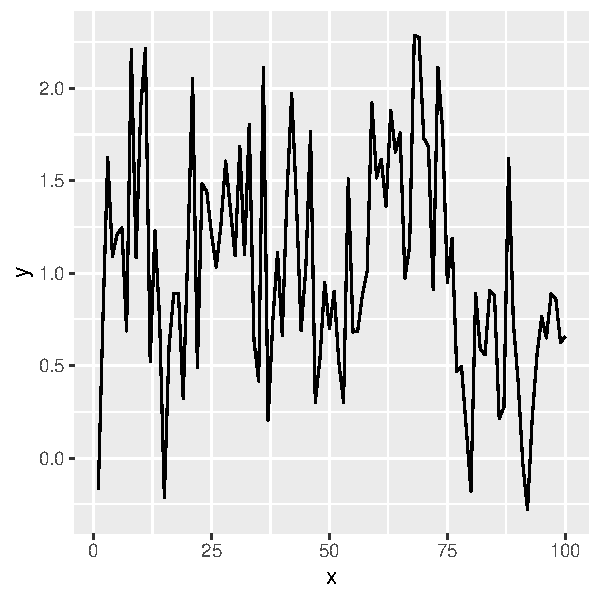
\includegraphics[keepaspectratio]{day2_practical_3_files/figure-pdf/unnamed-chunk-4-1.pdf}}
\end{center}

\subsubsection{\texorpdfstring{Fitting an AR(1) model with
\texttt{inlabru}}{Fitting an AR(1) model with inlabru}}\label{fitting-an-ar1-model-with-inlabru}

\textbf{Model components}

First, we define the model components, notice that the latent field is
defined by two components: the intercept \(\alpha\) and the
autoregressive random effects \(u_t\):

\begin{Shaded}
\begin{Highlighting}[]
\CommentTok{\# Model components}
\NormalTok{cmp }\OtherTok{=}  \ErrorTok{\textasciitilde{}} \SpecialCharTok{{-}}\DecValTok{1} \SpecialCharTok{+} \FunctionTok{alpha}\NormalTok{(}\DecValTok{1}\NormalTok{) }\SpecialCharTok{+} \FunctionTok{ut}\NormalTok{(x,}\AttributeTok{model =} \StringTok{"ar1"}\NormalTok{)}
\end{Highlighting}
\end{Shaded}

The we can define the formula for the linear predictor and specify the
observational model

\begin{Shaded}
\begin{Highlighting}[]
\CommentTok{\# Model formula}
\NormalTok{formula }\OtherTok{=}\NormalTok{ y }\SpecialCharTok{\textasciitilde{}}\NormalTok{ alpha }\SpecialCharTok{+}\NormalTok{ ut}
\CommentTok{\# Observational model}
\NormalTok{lik }\OtherTok{=}  \FunctionTok{bru\_obs}\NormalTok{(}\AttributeTok{formula =}\NormalTok{ y }\SpecialCharTok{\textasciitilde{}}\NormalTok{.,}
            \AttributeTok{family =} \StringTok{"gaussian"}\NormalTok{,}
            \AttributeTok{data =}\NormalTok{ ts\_dat)}
\end{Highlighting}
\end{Shaded}

Lastly, we fit the model using the \texttt{bru} function and compare the
model estimates with the true mdeol parameters we simulate our data
from.

\begin{Shaded}
\begin{Highlighting}[]
\CommentTok{\# fit the model}
\NormalTok{fit.ar1 }\OtherTok{=} \FunctionTok{bru}\NormalTok{(cmp, lik)}

\CommentTok{\# compare against the true values}

\FunctionTok{data.frame}\NormalTok{(}
  \AttributeTok{true =} \FunctionTok{c}\NormalTok{(a,tau\_e,marg.prec,phi),}
  \FunctionTok{rbind}\NormalTok{(fit.ar1}\SpecialCharTok{$}\NormalTok{summary.fixed[,}\FunctionTok{c}\NormalTok{(}\DecValTok{1}\NormalTok{,}\DecValTok{3}\NormalTok{,}\DecValTok{5}\NormalTok{)],}
\NormalTok{        fit.ar1}\SpecialCharTok{$}\NormalTok{summary.hyperpar[,}\FunctionTok{c}\NormalTok{(}\DecValTok{1}\NormalTok{,}\DecValTok{3}\NormalTok{,}\DecValTok{5}\NormalTok{)])}
\NormalTok{        ) }\SpecialCharTok{\%\textgreater{}\%} \FunctionTok{round}\NormalTok{(}\DecValTok{2}\NormalTok{)}
\end{Highlighting}
\end{Shaded}

\begin{verbatim}
                                        true mean X0.025quant X0.975quant
alpha                                    1.0 1.00        0.69        1.28
Precision for the Gaussian observations  5.0 4.91        3.11        7.29
Precision for ut                         3.6 7.96        2.91       18.10
Rho for ut                               0.8 0.80        0.54        0.94
\end{verbatim}

\textbf{Model predictions}

Here, we will predict the mean of our time series along with 95\%
credible intervals. Note that this interval are for the mean and not for
new observations, we will cover forecasting new observations next.

\begin{Shaded}
\begin{Highlighting}[]
\NormalTok{pred\_ar1 }\OtherTok{=} \FunctionTok{predict}\NormalTok{(fit.ar1, ts\_dat, }\SpecialCharTok{\textasciitilde{}}\NormalTok{ alpha }\SpecialCharTok{+}\NormalTok{ ut)}

\FunctionTok{ggplot}\NormalTok{(pred\_ar1,}\FunctionTok{aes}\NormalTok{(}\AttributeTok{y=}\NormalTok{mean,}\AttributeTok{x=}\NormalTok{x))}\SpecialCharTok{+}
  \FunctionTok{geom\_line}\NormalTok{()}\SpecialCharTok{+}
    \FunctionTok{geom\_ribbon}\NormalTok{(}\FunctionTok{aes}\NormalTok{(}\AttributeTok{x =}\NormalTok{ x, }\AttributeTok{y =}\NormalTok{ mean, }\AttributeTok{ymin =}\NormalTok{ q0}\FloatTok{.025}\NormalTok{, }\AttributeTok{ymax =}\NormalTok{ q0}\FloatTok{.975}\NormalTok{),}
                \AttributeTok{alpha =} \FloatTok{0.5}\NormalTok{) }\SpecialCharTok{+}
  \FunctionTok{geom\_point}\NormalTok{(}\FunctionTok{aes}\NormalTok{(}\AttributeTok{y=}\NormalTok{y,}\AttributeTok{x=}\NormalTok{x))}
\end{Highlighting}
\end{Shaded}

\pandocbounded{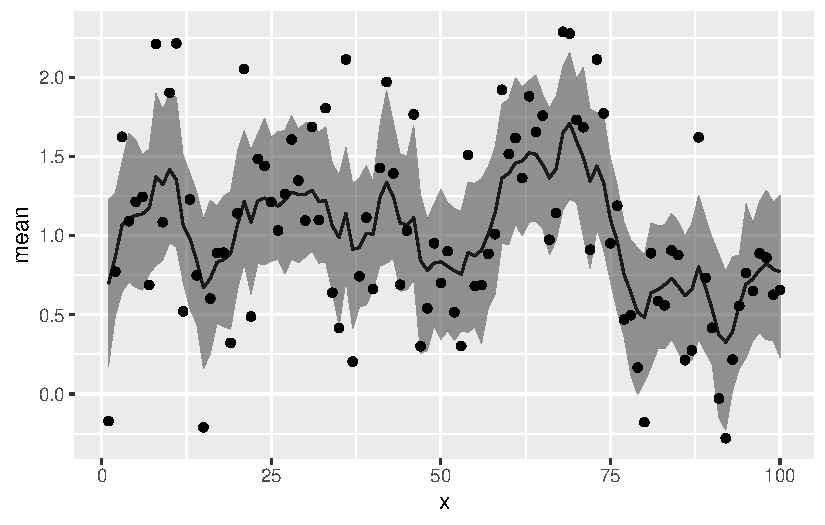
\includegraphics[keepaspectratio]{day2_practical_3_files/figure-pdf/unnamed-chunk-8-1.pdf}}

\subsubsection{\texorpdfstring{\textbf{Forecasting}}{Forecasting}}\label{forecasting}

A common goal in time series modelling is forecasting into the future.
Forecasting can be treated as a missing data problem where future values
of the response variable are missing. Let \(y_m\) be the missing
response, then, by fitting a statistical model to the observed data
\(\mathbf{y}_{obs}\), we condition on its parameters to obtain the
posterior predictive distribution:

\[
\pi(y_{m} \mid \mathbf{y}_{obs}) = \int \pi(y_{m}, \theta \mid \mathbf{y}_{obs})  d\theta = \int \pi(y_{m} \mid \mathbf{y}_{obs}, \theta) \pi(\theta \mid \mathbf{y}_{obs})  d\theta
\]

This distribution, which integrates over all parameter uncertainty,
provides the complete probabilistic forecast for the missing values.
\texttt{INLA} will automatically compute the predictive distributions
for all missing values in the response. To do so, we can augment our
data set by including the new time points at which the prediction will
be made and setting the response value to~\texttt{NA}~for these new time
points:

\begin{Shaded}
\begin{Highlighting}[]
\NormalTok{ts.forecast }\OtherTok{\textless{}{-}} \FunctionTok{rbind}\NormalTok{(ts\_dat, }
  \FunctionTok{data.frame}\NormalTok{(}\AttributeTok{y =} \FunctionTok{rep}\NormalTok{(}\ConstantTok{NA}\NormalTok{, }\DecValTok{50}\NormalTok{), }\AttributeTok{x =} \DecValTok{101}\SpecialCharTok{:}\DecValTok{150}\NormalTok{))}
\end{Highlighting}
\end{Shaded}

Next, we fit the~\texttt{ar1}~model to the new dataset so that the
predictive distributions are computed:

\begin{Shaded}
\begin{Highlighting}[]
\NormalTok{cmp }\OtherTok{=}  \ErrorTok{\textasciitilde{}} \SpecialCharTok{{-}}\DecValTok{1} \SpecialCharTok{+} \FunctionTok{alpha}\NormalTok{(}\DecValTok{1}\NormalTok{) }\SpecialCharTok{+} \FunctionTok{ut}\NormalTok{(x,}\AttributeTok{model =} \StringTok{"ar1"}\NormalTok{)}

\NormalTok{pred\_lik }\OtherTok{=}  \FunctionTok{bru\_obs}\NormalTok{(}\AttributeTok{formula =}\NormalTok{ y }\SpecialCharTok{\textasciitilde{}}\NormalTok{.,}
            \AttributeTok{family =} \StringTok{"gaussian"}\NormalTok{,}
            \AttributeTok{data =}\NormalTok{ ts.forecast)}

\NormalTok{fit.forecast }\OtherTok{=} \FunctionTok{bru}\NormalTok{(cmp, pred\_lik)}
\end{Highlighting}
\end{Shaded}

Lastly, we can draw samples from the posterior predictive distribution
using the \texttt{predict} function and visualize our forecast as
follows:

\begin{Shaded}
\begin{Highlighting}[]
\NormalTok{pred\_forecast }\OtherTok{=} \FunctionTok{predict}\NormalTok{(fit.forecast, ts.forecast, }\SpecialCharTok{\textasciitilde{}}\NormalTok{ alpha }\SpecialCharTok{+}\NormalTok{ ut)}

\NormalTok{p1}\OtherTok{=} \FunctionTok{ggplot}\NormalTok{(pred\_forecast,}\FunctionTok{aes}\NormalTok{(}\AttributeTok{y=}\NormalTok{mean,}\AttributeTok{x=}\NormalTok{x))}\SpecialCharTok{+}
  \FunctionTok{geom\_line}\NormalTok{()}\SpecialCharTok{+}
    \FunctionTok{geom\_ribbon}\NormalTok{(}\FunctionTok{aes}\NormalTok{(}\AttributeTok{x =}\NormalTok{ x, }\AttributeTok{y =}\NormalTok{ mean, }\AttributeTok{ymin =}\NormalTok{ q0}\FloatTok{.025}\NormalTok{, }\AttributeTok{ymax =}\NormalTok{ q0}\FloatTok{.975}\NormalTok{),}
                \AttributeTok{alpha =} \FloatTok{0.5}\NormalTok{) }\SpecialCharTok{+}
  \FunctionTok{geom\_point}\NormalTok{(}\AttributeTok{data=}\NormalTok{ts\_dat, }\FunctionTok{aes}\NormalTok{(}\AttributeTok{y=}\NormalTok{y,}\AttributeTok{x=}\NormalTok{x))}
\end{Highlighting}
\end{Shaded}

\subsection{Modelling Great Lakes water
level}\label{modelling-great-lakes-water-level}

In this exercise we will:

\begin{itemize}
\item
  Fit an AR(1) process with \texttt{inlabru} to model lakes water levels
\item
  Change the default priors for the observational error
\item
  Set penalized complexity priors for the correlation and precision
  parameters of the latent effects.
\item
  Fit a RW(1) model
\item
  Fit a an AR(1) model with group-level correlation
\end{itemize}

Start by loading useful libraries:

\begin{Shaded}
\begin{Highlighting}[]
\FunctionTok{library}\NormalTok{(tidyverse) }
\FunctionTok{library}\NormalTok{(INLA) }
\FunctionTok{library}\NormalTok{(ggplot2)}
\FunctionTok{library}\NormalTok{(patchwork) }
\FunctionTok{library}\NormalTok{(inlabru)}
\FunctionTok{library}\NormalTok{(DAAG)}
\end{Highlighting}
\end{Shaded}

In this exercise we will look at
\href{https://rdrr.io/cran/DAAG/man/greatLakes.html}{greatLakes} dataset
from the \texttt{DAAG} package. The data set contains the water level
heights for the lakes Erie, Michigan/Huron, Ontario and St Clair from
1918 to 2009.

Lets begin by loading and formatting the data into a tidy format.

\begin{Shaded}
\begin{Highlighting}[]
\FunctionTok{data}\NormalTok{(}\StringTok{"greatLakes"}\NormalTok{)}

\NormalTok{greatLakes.df }\OtherTok{=} \FunctionTok{data.frame}\NormalTok{(}\FunctionTok{as.matrix}\NormalTok{(greatLakes),}
                           \AttributeTok{year =} \FunctionTok{time}\NormalTok{(greatLakes)) }\SpecialCharTok{\%\textgreater{}\%}
  \FunctionTok{pivot\_longer}\NormalTok{(}\AttributeTok{cols =} \FunctionTok{c}\NormalTok{(}\StringTok{"Erie"}\NormalTok{,}\StringTok{"michHuron"}\NormalTok{,}\StringTok{"Ontario"}\NormalTok{,}\StringTok{"StClair"}\NormalTok{),}
               \AttributeTok{names\_to =} \StringTok{"Lakes"}\NormalTok{,}
               \AttributeTok{values\_to =} \StringTok{"height"}\NormalTok{ ) }
\end{Highlighting}
\end{Shaded}

\begin{center}
\pandocbounded{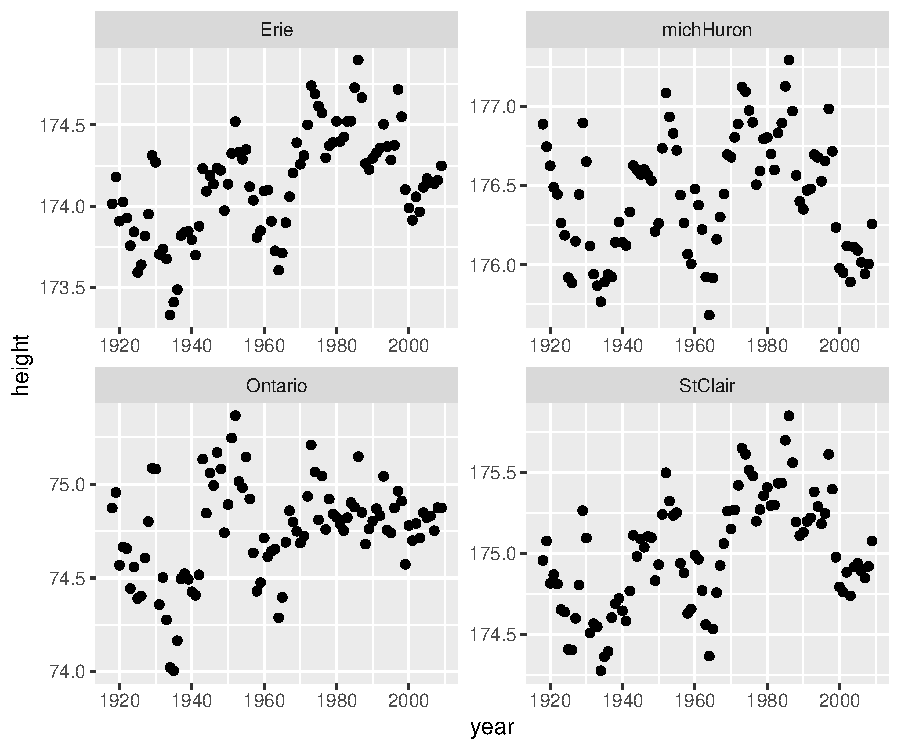
\includegraphics[keepaspectratio]{day2_practical_3_files/figure-pdf/unnamed-chunk-25-1.pdf}}
\end{center}

\subsubsection{\texorpdfstring{Fitting an AR(1) model in
\texttt{inlabru}}{Fitting an AR(1) model in inlabru}}\label{fitting-an-ar1-model-in-inlabru}

We will focus on the Erin lake for now. Lets begin by fitting an AR(1)
model of the form:

\[
\begin{aligned}
\text{height}_t &= \alpha + u_t +\varepsilon_t~; ~~ \varepsilon_t\sim \mathcal{N}(0,\tau_e^{-1}) \\
u_t &= \phi u_{t-1} + \delta_t~~~ ; ~~ \delta_t \sim \mathcal{N}(0,\tau_u^{-1}); ~~ t > 1 \\
x_1 &= \mathcal{N}(0,\kappa^{-1})\\
\kappa &= \tau_u (1-\phi^2)
\end{aligned}
\]

Where \(\alpha\) is the intercept, \(\phi\) is the correlation term,
\(\varepsilon\) is the observational Gaussian error with mean zero and
precision \(\tau_e\) and \(\kappa\) is the marginal precision for the
state \(u_t\) for \(t= 1,\ldots,92\).

First we make a subset of the dataset and create a time index \(T\):

\begin{Shaded}
\begin{Highlighting}[]
\NormalTok{greatLakes.df}\SpecialCharTok{$}\NormalTok{t.idx }\OtherTok{\textless{}{-}}\NormalTok{ greatLakes.df}\SpecialCharTok{$}\NormalTok{year}\DecValTok{{-}1917}

\NormalTok{Erie.df }\OtherTok{=}\NormalTok{ greatLakes.df }\SpecialCharTok{\%\textgreater{}\%} \FunctionTok{filter}\NormalTok{(Lakes }\SpecialCharTok{==} \StringTok{"Erie"}\NormalTok{)}
\end{Highlighting}
\end{Shaded}

\begin{tcolorbox}[enhanced jigsaw, colframe=quarto-callout-warning-color-frame, arc=.35mm, breakable, opacitybacktitle=0.6, toptitle=1mm, coltitle=black, toprule=.15mm, colbacktitle=quarto-callout-warning-color!10!white, leftrule=.75mm, colback=white, bottomtitle=1mm, titlerule=0mm, bottomrule=.15mm, title={Task}, opacityback=0, rightrule=.15mm, left=2mm]

Fit an AR(1) model to the Erie lake data using \texttt{inlabru}, then
plot the model fitted values showing 95\% credible intervals.

Take hint

Remember this is done by (1) defining the model components, (2) the
formula and (3) the observational model. Then you can use the
\texttt{predict} function to compute the predicted values for the mean
along with 95\% credible intervals.

Click here to see the solution

\begin{Shaded}
\begin{Highlighting}[]
\CommentTok{\# Model components}
\NormalTok{cmp }\OtherTok{=}  \ErrorTok{\textasciitilde{}} \SpecialCharTok{{-}}\DecValTok{1} \SpecialCharTok{+} \FunctionTok{alpha}\NormalTok{(}\DecValTok{1}\NormalTok{) }\SpecialCharTok{+} \FunctionTok{ut}\NormalTok{(t.idx,}\AttributeTok{model =} \StringTok{"ar1"}\NormalTok{)}
\CommentTok{\# Model formula}
\NormalTok{formula }\OtherTok{=}\NormalTok{ height }\SpecialCharTok{\textasciitilde{}}\NormalTok{ alpha }\SpecialCharTok{+}\NormalTok{ ut}


\CommentTok{\# Observational model}
\NormalTok{lik }\OtherTok{=}  \FunctionTok{bru\_obs}\NormalTok{(}\AttributeTok{formula =}\NormalTok{ height   }\SpecialCharTok{\textasciitilde{}}\NormalTok{.,}
            \AttributeTok{family =} \StringTok{"gaussian"}\NormalTok{,}
            \AttributeTok{data =}\NormalTok{ Erie.df )}

\CommentTok{\# fit the model}
\NormalTok{fit.Erie\_ar1 }\OtherTok{=} \FunctionTok{bru}\NormalTok{(cmp, lik)}

\CommentTok{\# Model predictions }

\NormalTok{pred\_ar1.Erie }\OtherTok{=} \FunctionTok{predict}\NormalTok{(fit.Erie\_ar1, Erie.df, }\SpecialCharTok{\textasciitilde{}}\NormalTok{ alpha }\SpecialCharTok{+}\NormalTok{ ut)}

\CommentTok{\# plot model fitted values}
\FunctionTok{ggplot}\NormalTok{(pred\_ar1.Erie,}\FunctionTok{aes}\NormalTok{(}\AttributeTok{y=}\NormalTok{mean,}\AttributeTok{x=}\NormalTok{year))}\SpecialCharTok{+}
  \FunctionTok{geom\_line}\NormalTok{()}\SpecialCharTok{+}
    \FunctionTok{geom\_ribbon}\NormalTok{(}\FunctionTok{aes}\NormalTok{(}\AttributeTok{x =}\NormalTok{ year, }\AttributeTok{y =}\NormalTok{ mean, }\AttributeTok{ymin =}\NormalTok{ q0}\FloatTok{.025}\NormalTok{, }\AttributeTok{ymax =}\NormalTok{ q0}\FloatTok{.975}\NormalTok{),}
                \AttributeTok{alpha =} \FloatTok{0.5}\NormalTok{) }\SpecialCharTok{+}
  \FunctionTok{geom\_point}\NormalTok{(}\FunctionTok{aes}\NormalTok{(}\AttributeTok{y=}\NormalTok{height,}\AttributeTok{x=}\NormalTok{year))}
\end{Highlighting}
\end{Shaded}

\begin{center}
\pandocbounded{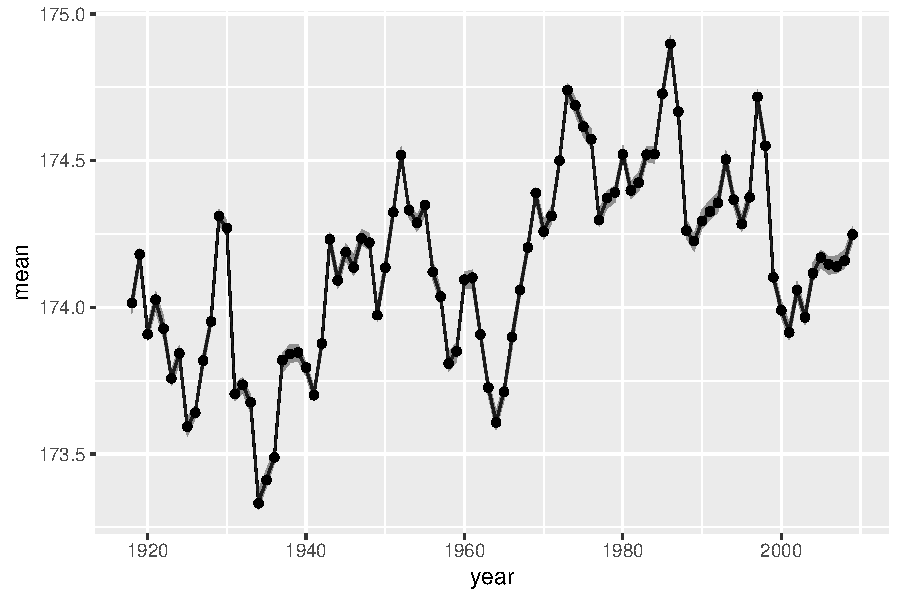
\includegraphics[keepaspectratio]{day2_practical_3_files/figure-pdf/unnamed-chunk-27-1.pdf}}
\end{center}

\end{tcolorbox}

\begin{tcolorbox}[enhanced jigsaw, colframe=quarto-callout-tip-color-frame, arc=.35mm, breakable, opacitybacktitle=0.6, toptitle=1mm, coltitle=black, toprule=.15mm, colbacktitle=quarto-callout-tip-color!10!white, leftrule=.75mm, colback=white, bottomtitle=1mm, titlerule=0mm, bottomrule=.15mm, title={Question}, opacityback=0, rightrule=.15mm, left=2mm]

Are there any issues with the fitted model, and if so, how do you think
we should address them?

Answer

It is clear that the model overfits the data, leading to poor predictive
performance. Thus, we need to introduce some prior information on the
what we expect the variation of the process to be.

\end{tcolorbox}

\textbf{Priors}

Let review INLA' prior parametrization for autoregressive models:

Let \(\pmb{\theta} = \{\theta_y,\theta_u,\theta_\phi\}\) be INLA's
internal representation of the hyperparameters such that:

\(\theta_y = \log(\tau^2_y)\)

\(\theta_u = \log(\kappa) = \log\left(\tau_u[1-\phi^2]\right)\)

\(\theta_\phi = \log \left(\frac{1+\phi}{1-\phi}\right)\)

The default priors for \(\{\theta_y,\theta_u\}\) are
\(\text{log-gamma} (1, 5\times 10^{-5} )\) priors with default initial
values set to 4 in each case. Then, Gaussian priors
\(\alpha \sim \mathcal{N}(0,\tau_y = 0.001)\) and
\(\theta_\phi \sim \mathcal{N}(0, \tau_y= 0.15)\) are used for the
intercept and correlation parameter respectively.

\begin{tcolorbox}[enhanced jigsaw, colframe=quarto-callout-note-color-frame, arc=.35mm, breakable, opacitybacktitle=0.6, toptitle=1mm, coltitle=black, toprule=.15mm, colbacktitle=quarto-callout-note-color!10!white, leftrule=.75mm, colback=white, bottomtitle=1mm, titlerule=0mm, bottomrule=.15mm, title=\textcolor{quarto-callout-note-color}{\faInfo}\hspace{0.5em}{Note}, opacityback=0, rightrule=.15mm, left=2mm]

Specifically for AR(1) correlation parameter \(\phi\), INLA uses the
following logit transformation on \(\theta_\phi\):

\[ \phi = \frac{2\exp(\theta_\phi)}{1+ \exp(\theta_\phi)} -1. \]

\end{tcolorbox}

\textbf{Setting priors and PC-priors}

Lets now set a Gamma prior with parameters 1 and 1, so that the
precision of the Gaussian osbervational error is centered at 1 with a
variance of 1. Additionally we will set Penalized Complexity (PC) priors
according to the following probability statements:

\begin{itemize}
\item
  \(P(\sigma > 1) = 0.01\)
\item
  \(P(\phi > 0.5) = 0.3\)
\end{itemize}

Notice that the PC prior for the precision \(\tau_u\) is defined on the
standard deviation \(\sigma_u = \tau_u^{-1/2}\)

\begin{Shaded}
\begin{Highlighting}[]
\NormalTok{pc\_prior }\OtherTok{\textless{}{-}} \FunctionTok{list}\NormalTok{(}\AttributeTok{theta =} \FunctionTok{list}\NormalTok{(}\AttributeTok{prior =} \StringTok{"pc.prec"}\NormalTok{, }\AttributeTok{param =} \FunctionTok{c}\NormalTok{(}\DecValTok{1}\NormalTok{, }\FloatTok{0.01}\NormalTok{)),}
                 \AttributeTok{rho =} \FunctionTok{list}\NormalTok{(}\AttributeTok{prior =} \StringTok{"pc.cor0"}\NormalTok{, }\AttributeTok{param =} \FunctionTok{c}\NormalTok{(}\FloatTok{0.5}\NormalTok{, }\FloatTok{0.3}\NormalTok{))) }

\NormalTok{prec.tau\_e }\OtherTok{\textless{}{-}} \FunctionTok{list}\NormalTok{(}\AttributeTok{prec =} \FunctionTok{list}\NormalTok{(}\AttributeTok{prior =} \StringTok{"loggamma"}\NormalTok{,   }\CommentTok{\# prior name}
                             \AttributeTok{param =} \FunctionTok{c}\NormalTok{(}\DecValTok{1}\NormalTok{, }\DecValTok{1}\NormalTok{))) }\CommentTok{\# prior values}

\CommentTok{\# Model components}
\NormalTok{cmp }\OtherTok{=}  \ErrorTok{\textasciitilde{}} \SpecialCharTok{{-}}\DecValTok{1} \SpecialCharTok{+} \FunctionTok{alpha}\NormalTok{(}\DecValTok{1}\NormalTok{) }\SpecialCharTok{+} \FunctionTok{ut}\NormalTok{(t.idx, }\AttributeTok{model =} \StringTok{"ar1"}\NormalTok{,  }\AttributeTok{hyper =}\NormalTok{ pc\_prior)}
\CommentTok{\# Model formula}
\NormalTok{formula }\OtherTok{=}\NormalTok{ height }\SpecialCharTok{\textasciitilde{}}\NormalTok{ alpha }\SpecialCharTok{+}\NormalTok{ ut}


\CommentTok{\# Observational model}
\NormalTok{lik }\OtherTok{=}  \FunctionTok{bru\_obs}\NormalTok{(}\AttributeTok{formula =}\NormalTok{ height  }\SpecialCharTok{\textasciitilde{}}\NormalTok{.,}
            \AttributeTok{family =} \StringTok{"gaussian"}\NormalTok{,}
            \AttributeTok{data =}\NormalTok{ Erie.df,}
            \AttributeTok{control.family =} \FunctionTok{list}\NormalTok{(}\AttributeTok{hyper =}\NormalTok{ prec.tau\_e))}

\CommentTok{\# fit the model}
\NormalTok{fit.Erie\_ar1 }\OtherTok{=} \FunctionTok{bru}\NormalTok{(cmp, lik)}
\end{Highlighting}
\end{Shaded}

\begin{tcolorbox}[enhanced jigsaw, colframe=quarto-callout-tip-color-frame, arc=.35mm, breakable, opacitybacktitle=0.6, toptitle=1mm, coltitle=black, toprule=.15mm, colbacktitle=quarto-callout-tip-color!10!white, leftrule=.75mm, colback=white, bottomtitle=1mm, titlerule=0mm, bottomrule=.15mm, title={Question}, opacityback=0, rightrule=.15mm, left=2mm]

What is the posterior mean for the correlation parameter \(\rho\)?
\_\_\_\_\_\_\_\_\_\_\_\_\_\_\_\_\_

\end{tcolorbox}

\begin{tcolorbox}[enhanced jigsaw, colframe=quarto-callout-warning-color-frame, arc=.35mm, breakable, opacitybacktitle=0.6, toptitle=1mm, coltitle=black, toprule=.15mm, colbacktitle=quarto-callout-warning-color!10!white, leftrule=.75mm, colback=white, bottomtitle=1mm, titlerule=0mm, bottomrule=.15mm, title={Task}, opacityback=0, rightrule=.15mm, left=2mm]

Plot the fitted values of the model, has the overfitting problem being
alleviated?

Click here to see the solution

\begin{center}
\pandocbounded{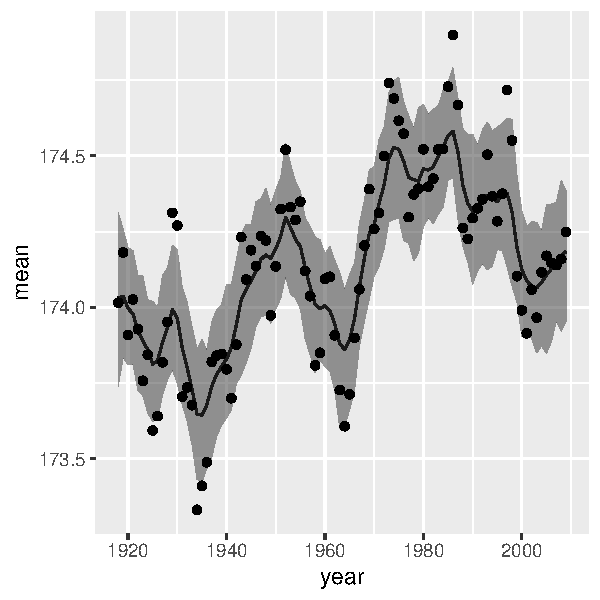
\includegraphics[keepaspectratio]{day2_practical_3_files/figure-pdf/unnamed-chunk-29-1.pdf}}
\end{center}

\end{tcolorbox}

\subsubsection{Fitting a RW(1) model}\label{fitting-a-rw1-model}

Now we fit a random walk of order 1 to the Erie lake data:

\[
\begin{aligned}
y_t &= \alpha + u_t + \varepsilon_t, ~ t = 1,\ldots,92 \\
 \varepsilon_t & \sim \mathcal{N}(0,\tau_e) \\
u_t - u_{t-1} &\sim \mathcal{N}(0,\tau_u),~ t = 2,\ldots,92 \\
\end{aligned}
\]

Firs we define model priors:

\begin{Shaded}
\begin{Highlighting}[]
\NormalTok{pc\_prior }\OtherTok{\textless{}{-}} \FunctionTok{list}\NormalTok{(}\AttributeTok{theta =} \FunctionTok{list}\NormalTok{(}\AttributeTok{prior =} \StringTok{"pc.prec"}\NormalTok{, }\AttributeTok{param =} \FunctionTok{c}\NormalTok{(}\DecValTok{1}\NormalTok{, }\FloatTok{0.01}\NormalTok{))) }

\NormalTok{prec.tau\_e }\OtherTok{\textless{}{-}} \FunctionTok{list}\NormalTok{(}\AttributeTok{prec =} \FunctionTok{list}\NormalTok{(}\AttributeTok{prior =} \StringTok{"loggamma"}\NormalTok{,   }\CommentTok{\# prior name}
                             \AttributeTok{param =} \FunctionTok{c}\NormalTok{(}\DecValTok{1}\NormalTok{, }\DecValTok{1}\NormalTok{))) }\CommentTok{\# prior values}
\end{Highlighting}
\end{Shaded}

Now we define model components:

\begin{Shaded}
\begin{Highlighting}[]
\NormalTok{cmp\_rw }\OtherTok{=}  \ErrorTok{\textasciitilde{}} \SpecialCharTok{{-}}\DecValTok{1} \SpecialCharTok{+} \FunctionTok{alpha}\NormalTok{(}\DecValTok{1}\NormalTok{) }\SpecialCharTok{+} 
  \FunctionTok{ut}\NormalTok{(t.idx ,}
     \AttributeTok{constr=}\ConstantTok{FALSE}\NormalTok{,}
     \AttributeTok{model =} \StringTok{"rw1"}\NormalTok{,}
     \AttributeTok{hyper=}\NormalTok{pc\_prior,}
     \AttributeTok{scale.model =} \ConstantTok{TRUE}\NormalTok{)}
\end{Highlighting}
\end{Shaded}

Notice that we have set \texttt{scale.model\ =\ TRUE} to scale the
latent effects. This is particularly important when Intrinsic Gaussian
Markov random fields (IGMRFs) are used as priors (e.g., random walk
models or some spatial models) for the latent effects. By defining
\texttt{scale.model\ =\ TRUE}, the \texttt{rw1}-model is scaled to have
a generalized variance equal to one. By scaling scaling the models we
ensure that a fixed hyperprior for the precision parameter has a similar
interpretation for different types of IGMRFs, making precision estimates
comparable between different models. Scaling also allows estimates to be
less sensitive to re-scaling covariates in the linear predictor and
makes the precision invariant to changes in the shape and size of the
latent effect (see Sørbye
(\href{https://www.sciencedirect.com/science/article/pii/S2211675313000407}{2014})
for further details) .

We can now fit the model with the updated components and plot the
predicted values

\begin{Shaded}
\begin{Highlighting}[]
\CommentTok{\# Model formula}
\NormalTok{formula }\OtherTok{=}\NormalTok{ height }\SpecialCharTok{\textasciitilde{}}\NormalTok{ alpha }\SpecialCharTok{+}\NormalTok{ ut}
\CommentTok{\# Observational model}
\NormalTok{lik }\OtherTok{=}  \FunctionTok{bru\_obs}\NormalTok{(}\AttributeTok{formula =}\NormalTok{ height  }\SpecialCharTok{\textasciitilde{}}\NormalTok{.,}
            \AttributeTok{family =} \StringTok{"gaussian"}\NormalTok{,}
            \AttributeTok{data =}\NormalTok{ Erie.df,}
            \AttributeTok{control.family =} \FunctionTok{list}\NormalTok{(}\AttributeTok{hyper =}\NormalTok{ prec.tau\_e))}
\CommentTok{\# fit the model}
\NormalTok{fit.Erie\_rw1 }\OtherTok{=} \FunctionTok{bru}\NormalTok{(cmp\_rw, lik)}
\CommentTok{\# Model predictions}
\NormalTok{pred\_rw1.Erie }\OtherTok{=} \FunctionTok{predict}\NormalTok{(fit.Erie\_rw1, Erie.df, }\SpecialCharTok{\textasciitilde{}}\NormalTok{ alpha }\SpecialCharTok{+}\NormalTok{ ut)}
\end{Highlighting}
\end{Shaded}

\begin{center}
\pandocbounded{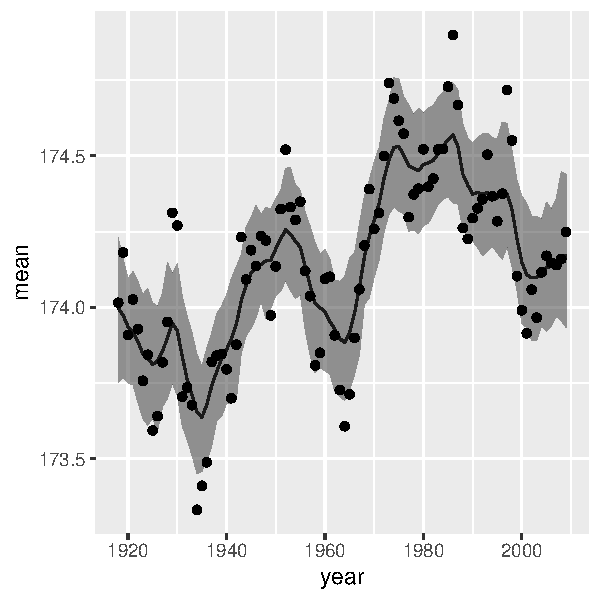
\includegraphics[keepaspectratio]{day2_practical_3_files/figure-pdf/unnamed-chunk-33-1.pdf}}
\end{center}

\begin{tcolorbox}[enhanced jigsaw, colframe=quarto-callout-tip-color-frame, arc=.35mm, breakable, opacitybacktitle=0.6, toptitle=1mm, coltitle=black, toprule=.15mm, colbacktitle=quarto-callout-tip-color!10!white, leftrule=.75mm, colback=white, bottomtitle=1mm, titlerule=0mm, bottomrule=.15mm, title={Question}, opacityback=0, rightrule=.15mm, left=2mm]

Take a look at the model summaries using the \texttt{summary} function,
do you see anything odd?

Answer

The intercept has zero mean and a very large variance. This is because
we have not imposed a sum-to-zero constraint on the model random effects
(\texttt{constr=FALSE}). Without this constraint, intrinsic models are
non-identifiable. The intercept and the random effects are confounded,
For example, you could add a constant value to every random effect and
subtract it from the intercept without changing the model's predictions.
Take for instance for any constant \(c\), the following models are
identical:

\(y_t = \alpha + u_{t} + \varepsilon_t\)
\(y_t = (\alpha - c) + (u_{t} + c) + \varepsilon_t\)

Thus, you need to set \texttt{constr=FALSE} so that \(\sum_t u_t=0\) to
ensure identifiability of \(\alpha\)

\end{tcolorbox}

\begin{tcolorbox}[enhanced jigsaw, colframe=quarto-callout-warning-color-frame, arc=.35mm, breakable, opacitybacktitle=0.6, toptitle=1mm, coltitle=black, toprule=.15mm, colbacktitle=quarto-callout-warning-color!10!white, leftrule=.75mm, colback=white, bottomtitle=1mm, titlerule=0mm, bottomrule=.15mm, title={Task}, opacityback=0, rightrule=.15mm, left=2mm]

Fit an RW(1) model to the Erie data but now set \texttt{constr=TRUE} to
impose a sum-to-zero constraint on the random effect. Then compare your
results with the unconstrained model.

Click here to see the solution

\begin{Shaded}
\begin{Highlighting}[]
\CommentTok{\# Model components}
\NormalTok{cmp\_rw }\OtherTok{=}  \ErrorTok{\textasciitilde{}} \SpecialCharTok{{-}}\DecValTok{1} \SpecialCharTok{+} \FunctionTok{alpha}\NormalTok{(}\DecValTok{1}\NormalTok{) }\SpecialCharTok{+} 
  \FunctionTok{ut}\NormalTok{(t.idx ,}
     \AttributeTok{constr=}\ConstantTok{TRUE}\NormalTok{,}
     \AttributeTok{model =} \StringTok{"rw1"}\NormalTok{,}
     \AttributeTok{hyper=}\NormalTok{pc\_prior,}
     \AttributeTok{scale.model =} \ConstantTok{TRUE}\NormalTok{)}

\NormalTok{fit.Erie\_rw1\_constr }\OtherTok{=} \FunctionTok{bru}\NormalTok{(cmp\_rw, lik)}

\NormalTok{fit.Erie\_rw1\_constr}\SpecialCharTok{$}\NormalTok{summary.fixed}
\end{Highlighting}
\end{Shaded}

\begin{verbatim}
          mean         sd 0.025quant 0.5quant 0.975quant     mode          kld
alpha 174.1381 0.02383785   174.0913 174.1381    174.185 174.1381 1.440666e-08
\end{verbatim}

\end{tcolorbox}

\subsubsection{Group-level effects}\label{group-level-effects}

Now we will model the height water levels for all four lakes by grouping
the random effects. This will allow a within-lakes correlation to be
included. In the next example, we allow for correlated effects using an
\texttt{ar1} model for the years and \texttt{iid} random effects on the
lakes. First we create a lakes id and set the priors for our model:

\begin{Shaded}
\begin{Highlighting}[]
\NormalTok{greatLakes.df}\SpecialCharTok{$}\NormalTok{lake\_id }\OtherTok{\textless{}{-}} \FunctionTok{as.numeric}\NormalTok{(}\FunctionTok{as.factor}\NormalTok{(greatLakes.df}\SpecialCharTok{$}\NormalTok{Lakes))}

\NormalTok{pc\_prior }\OtherTok{\textless{}{-}} \FunctionTok{list}\NormalTok{(}\AttributeTok{theta =} \FunctionTok{list}\NormalTok{(}\AttributeTok{prior =} \StringTok{"pc.prec"}\NormalTok{, }\AttributeTok{param =} \FunctionTok{c}\NormalTok{(}\DecValTok{1}\NormalTok{, }\FloatTok{0.01}\NormalTok{)),}
                 \AttributeTok{rho =} \FunctionTok{list}\NormalTok{(}\AttributeTok{prior =} \StringTok{"pc.cor0"}\NormalTok{, }\AttributeTok{param =} \FunctionTok{c}\NormalTok{(}\FloatTok{0.5}\NormalTok{, }\FloatTok{0.3}\NormalTok{))) }

\NormalTok{prec.tau\_e }\OtherTok{\textless{}{-}} \FunctionTok{list}\NormalTok{(}\AttributeTok{prec =} \FunctionTok{list}\NormalTok{(}\AttributeTok{prior =} \StringTok{"loggamma"}\NormalTok{,   }\CommentTok{\# prior name}
                             \AttributeTok{param =} \FunctionTok{c}\NormalTok{(}\DecValTok{1}\NormalTok{, }\DecValTok{10}\NormalTok{))) }\CommentTok{\# prior values}
\end{Highlighting}
\end{Shaded}

Now we define the model components. The lakes IDs that define the group
are passed with parameter \texttt{group} argument and the \texttt{iid}
model and other parameters are passed through the \texttt{control.group}
parameter.

\begin{Shaded}
\begin{Highlighting}[]
\CommentTok{\# Model components}
\NormalTok{cmp }\OtherTok{=}  \ErrorTok{\textasciitilde{}} \SpecialCharTok{{-}}\DecValTok{1} \SpecialCharTok{+} \FunctionTok{alpha}\NormalTok{(}\DecValTok{1}\NormalTok{) }\SpecialCharTok{+} \FunctionTok{ut}\NormalTok{(year,}\AttributeTok{model =} \StringTok{"ar1"}\NormalTok{,}
                            \AttributeTok{hyper =}\NormalTok{ pc\_prior,}
                            \AttributeTok{group =}\NormalTok{lake\_id,}
                            \AttributeTok{control.group =} 
                            \FunctionTok{list}\NormalTok{(}\AttributeTok{model =} \StringTok{"iid"}\NormalTok{, }
                                 \AttributeTok{scale.model =} \ConstantTok{TRUE}\NormalTok{))}
\end{Highlighting}
\end{Shaded}

We fit the model in a similar fashion as we did before:

\begin{Shaded}
\begin{Highlighting}[]
\CommentTok{\# Model formula}
\NormalTok{formula }\OtherTok{=}\NormalTok{ height }\SpecialCharTok{\textasciitilde{}}\NormalTok{ alpha }\SpecialCharTok{+}\NormalTok{ ut}


\CommentTok{\# Observational model}
\NormalTok{lik }\OtherTok{=}  \FunctionTok{bru\_obs}\NormalTok{(}\AttributeTok{formula =}\NormalTok{ height  }\SpecialCharTok{\textasciitilde{}}\NormalTok{.,}
            \AttributeTok{family =} \StringTok{"gaussian"}\NormalTok{,}
            \AttributeTok{data =}\NormalTok{ greatLakes.df,}
            \AttributeTok{control.family =} \FunctionTok{list}\NormalTok{(}\AttributeTok{hyper =}\NormalTok{ prec.tau\_e))}

\CommentTok{\# fit the model}
\NormalTok{fit.all\_lakes\_ar1 }\OtherTok{=} \FunctionTok{bru}\NormalTok{(cmp, lik)}

\CommentTok{\# Model predictions}
\NormalTok{pred\_ar1.all }\OtherTok{=} \FunctionTok{predict}\NormalTok{(fit.all\_lakes\_ar1, greatLakes.df, }\SpecialCharTok{\textasciitilde{}}\NormalTok{ alpha }\SpecialCharTok{+}\NormalTok{ ut)}
\end{Highlighting}
\end{Shaded}

Lastly we can visualize group-level model predictions as follows:

\begin{Shaded}
\begin{Highlighting}[]
\FunctionTok{ggplot}\NormalTok{(pred\_ar1.all,}\FunctionTok{aes}\NormalTok{(}\AttributeTok{y=}\NormalTok{mean,}\AttributeTok{x=}\NormalTok{year))}\SpecialCharTok{+}
  \FunctionTok{geom\_line}\NormalTok{()}\SpecialCharTok{+}
    \FunctionTok{geom\_ribbon}\NormalTok{(}\FunctionTok{aes}\NormalTok{(}\AttributeTok{x =}\NormalTok{ year, }\AttributeTok{y =}\NormalTok{ mean, }\AttributeTok{ymin =}\NormalTok{ q0}\FloatTok{.025}\NormalTok{, }\AttributeTok{ymax =}\NormalTok{ q0}\FloatTok{.975}\NormalTok{),}
                \AttributeTok{alpha =} \FloatTok{0.5}\NormalTok{) }\SpecialCharTok{+}
  \FunctionTok{geom\_point}\NormalTok{(}\FunctionTok{aes}\NormalTok{(}\AttributeTok{y=}\NormalTok{height,}\AttributeTok{x=}\NormalTok{year)) }\SpecialCharTok{+} \FunctionTok{facet\_wrap}\NormalTok{(}\SpecialCharTok{\textasciitilde{}}\NormalTok{Lakes,}\AttributeTok{scales =} \StringTok{"free"}\NormalTok{)}
\end{Highlighting}
\end{Shaded}

\pandocbounded{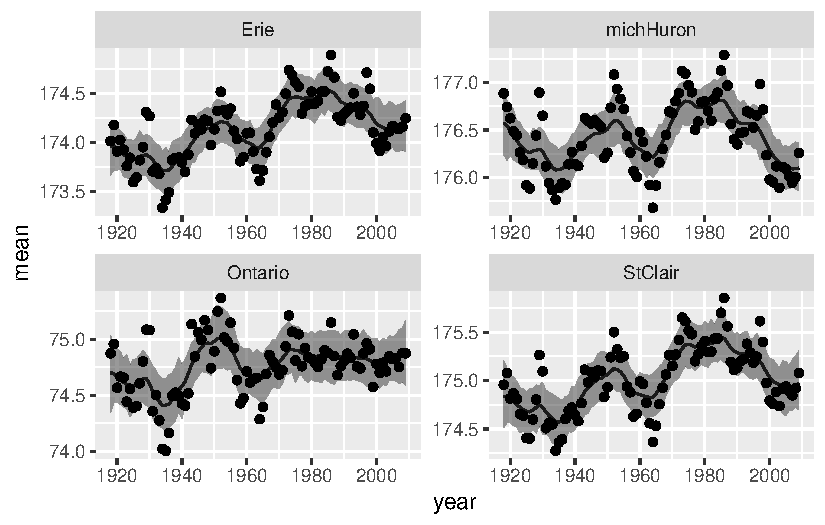
\includegraphics[keepaspectratio]{day2_practical_3_files/figure-pdf/unnamed-chunk-38-1.pdf}}

\subsection{Non-Gaussian data}\label{non-gaussian-data}

In the next example we will use the \texttt{Toyo} data set to illustrate
how temporal models can be fit to non-Gaussian data.

The \texttt{Tokyo} data set available in \texttt{INLA} contains the
recorded days of rain above 1 mm in Tokyo for 2 years, 1983:84. The data
set contains the following variables:

\begin{itemize}
\item
  \texttt{y} : number of days with rain
\item
  \texttt{n} : total number of days
\item
  \texttt{time} : day of the year
\end{itemize}

\begin{Shaded}
\begin{Highlighting}[]
\FunctionTok{library}\NormalTok{(INLA)}
\FunctionTok{library}\NormalTok{(inlabru)}
\FunctionTok{library}\NormalTok{(ggplot2)}
\FunctionTok{library}\NormalTok{(tidyr)}


\FunctionTok{data}\NormalTok{(}\StringTok{"Tokyo"}\NormalTok{)}
\end{Highlighting}
\end{Shaded}

A possible observational model for these data is

\[
\begin{aligned}
y_t|\eta_t & \sim\text{Bin}(n_t, p_t) \\
\eta_t &= \text{logit}(p_t),\qquad i = 1,\dots,366
\end{aligned}
\]

\[
n_t = \left\{
 \begin{array}{lr}
1, & \text{for}\; 29\; \text{February}\\
2, & \text{other days}
\end{array}\right.
\]

\[
y_t =
\begin{cases}
\{0,1\}, & \text{for}\; 29\; \text{February}\\
\{0,1,2\}, & \text{other days}
 \end{cases}
\]

Then, the latent field is given by

\[
\eta_t = \beta_0 + f(\text{time}_t)
\]

\begin{itemize}
\item
  Where the probability of rain depends on on the day of the year \(t\)
\item
  \(\beta_0\) is an intercept
\item
  \(f(\text{time}_t)\) is a temporal model, e.g., a RW2 model (this is
  just a smoother).
\end{itemize}

The smoothness is controlled by a hyperparameter \(\tau_f\) . Thus, we
assign a prior to \(\tau_f\) to finalize the model.

We can fit the model as follows:

\begin{Shaded}
\begin{Highlighting}[]
\CommentTok{\# define model component}
\NormalTok{cmp }\OtherTok{=}  \ErrorTok{\textasciitilde{}} \SpecialCharTok{{-}}\DecValTok{1} \SpecialCharTok{+} \FunctionTok{beta0}\NormalTok{(}\DecValTok{1}\NormalTok{) }\SpecialCharTok{+} \FunctionTok{time\_effect}\NormalTok{(time, }\AttributeTok{model =} \StringTok{"rw2"}\NormalTok{, }\AttributeTok{cyclic =} \ConstantTok{TRUE}\NormalTok{)}

\CommentTok{\# define model predictor}
\NormalTok{eta }\OtherTok{=}\NormalTok{ y }\SpecialCharTok{\textasciitilde{}}\NormalTok{ beta0 }\SpecialCharTok{+}\NormalTok{ time\_effect}

\CommentTok{\# build the observation model}
\NormalTok{lik }\OtherTok{=} \FunctionTok{bru\_obs}\NormalTok{(}\AttributeTok{formula =}\NormalTok{ eta,}
              \AttributeTok{family =} \StringTok{"binomial"}\NormalTok{,}
              \AttributeTok{Ntrials =}\NormalTok{ n,}
              \AttributeTok{data =}\NormalTok{ Tokyo)}

\CommentTok{\# fit the model}
\NormalTok{fit }\OtherTok{=} \FunctionTok{bru}\NormalTok{(cmp, lik)}
\end{Highlighting}
\end{Shaded}

Notice that we have set \texttt{cyclic\ =\ TRUE} as this is a cyclic
effect. Finally, we can produce model predictions in a similar fashion
as we did before:

\begin{Shaded}
\begin{Highlighting}[]
\NormalTok{pTokyo }\OtherTok{=} \FunctionTok{predict}\NormalTok{(fit, Tokyo, }\SpecialCharTok{\textasciitilde{}} \FunctionTok{plogis}\NormalTok{(beta0 }\SpecialCharTok{+}\NormalTok{ time\_effect))}

\FunctionTok{ggplot}\NormalTok{(}\AttributeTok{data=}\NormalTok{pTokyo , }\FunctionTok{aes}\NormalTok{(}\AttributeTok{x=}\NormalTok{ time, }\AttributeTok{y=}\NormalTok{ y) ) }\SpecialCharTok{+}
  \FunctionTok{geom\_point}\NormalTok{() }\SpecialCharTok{+} 
  \FunctionTok{ylab}\NormalTok{(}\StringTok{""}\NormalTok{) }\SpecialCharTok{+} \FunctionTok{xlab}\NormalTok{(}\StringTok{""}\NormalTok{) }\SpecialCharTok{+}
  \CommentTok{\# Custom the Y scales:}
  \FunctionTok{scale\_y\_continuous}\NormalTok{(}
    \CommentTok{\# Features of the first axis}
    \AttributeTok{name =} \StringTok{""}\NormalTok{,}
    \CommentTok{\# Add a second axis and specify its features}
    \AttributeTok{sec.axis =} \FunctionTok{sec\_axis}\NormalTok{( }\AttributeTok{transform=}\SpecialCharTok{\textasciitilde{}}\NormalTok{.}\SpecialCharTok{/}\DecValTok{2}\NormalTok{, }\AttributeTok{name=}\StringTok{"Probability"}\NormalTok{)}
\NormalTok{  )  }\SpecialCharTok{+} \FunctionTok{geom\_line}\NormalTok{(}\FunctionTok{aes}\NormalTok{(}\AttributeTok{y=}\NormalTok{mean}\SpecialCharTok{*}\DecValTok{2}\NormalTok{,}\AttributeTok{x=}\NormalTok{time)) }\SpecialCharTok{+}
  \FunctionTok{geom\_ribbon}\NormalTok{(}\FunctionTok{aes}\NormalTok{( }\AttributeTok{ymin =}\NormalTok{ q0}\FloatTok{.025}\SpecialCharTok{*}\DecValTok{2}\NormalTok{, }
                             \AttributeTok{ymax =}\NormalTok{ q0}\FloatTok{.975}\SpecialCharTok{*}\DecValTok{2}\NormalTok{), }\AttributeTok{alpha =} \FloatTok{0.5}\NormalTok{)}
\end{Highlighting}
\end{Shaded}

\pandocbounded{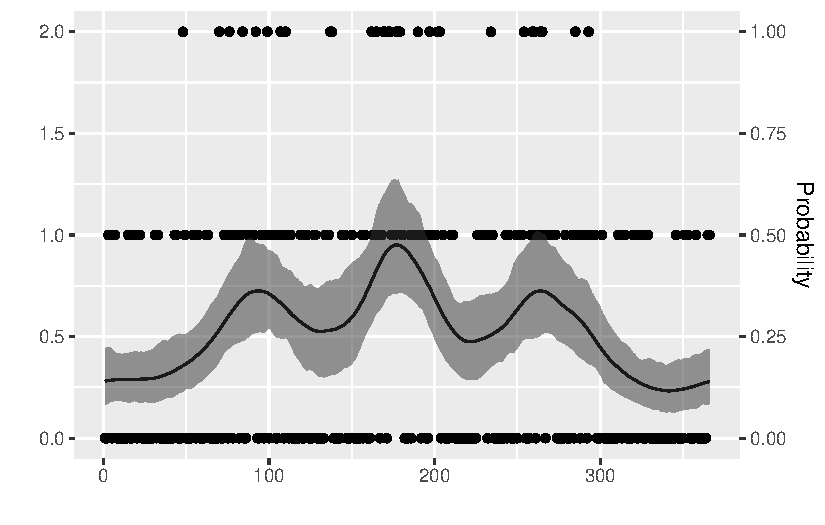
\includegraphics[keepaspectratio]{day2_practical_3_files/figure-pdf/unnamed-chunk-59-1.pdf}}




\end{document}
